%%%%%%%%%%%%%%%%%%%%%%%%%%%%%%%%%%%%%%%%%%%%%%%%%%%%%%%%%%%%%%%%%%%%%%%%
\chapter{La fattorizzazione CP}
%%%%%%%%%%%%%%%%%%%%%%%%%%%%%%%%%%%%%%%%%%%%%%%%%%%%%%%%%%%%%%%%%%%%%%%%

\todo{Usare emph quando si introduce un termine nuovo, inserire tabella notazione all'inizio}

\section{Tensori}

In questo elaborato lavoriamo in $ \K \in \{\R, \C\}  $, e denotiamo gli spazi vettoriali, che
assumeremo sempre finiti, con le lettere $  A, B, C, V, W$ e $A_j$, e le dimensioni con le
lettere $ \bm{a}, \bm{b}, \bm{c} $, etc. Dati dei vettori $ v_1,\ldots,v_p \in V$, l'insieme
$ \angb{v_1,\ldots,v_p} \subseteq V $ denota lo span lineare di $ v_1, \ldots, v_p $. Indichiamo con $ V^* = \{ f : V \to \K \mid f \text{ lineare} \} $ lo \emph{spazio duale} dello spazio $ V $, e per ogni $ \alpha \in V^* $, denotiamo con $
	\alpha^\perp = \{v \in V \mid \alpha(v) = 0\}  $ l'\emph{annullatore} di $ \alpha $. Similmente,
dato un sottospazio vettoriale $ U \subseteq V $, definiamo l'annullatore di $ U $ come $ U^\perp =
	\{\alpha \in V^* \mid \alpha(u) = 0, \, \forall u \in U\}  $.

\begin{definition}[Mappe trilineari]
	Siano $ U,V,W $ spazi vettoriali di dimensione finita su un campo $ \K $. Una \emph{forma bilineare} è una mappa $ \varphi : U \times V \to
		W$ lineare in ogni componente, in altre parole tale che $ f(u, \cdot) $ e $ f(\cdot,v) $ sono
	lineari per ogni $ u\in U $ e $ v\in V $. Quando $ W = \K $ la chiameremo \emph{forma bilineare}.



\end{definition}
In generale, dati degli spazi vettoriali $ A_1, \ldots, A_{n} $ di
dimensione finita, definiamo le forme $ n $-multilineari come applicazioni $ \varphi : A_1
	\times \cdots \times A_{n} \to \K $ lineari in ognuna delle $ n $ componenti, e data una forma $ n
$-multilineare $ \varphi : A_1 \times A_2 \times \cdots \times A_{n} $ è possibile costruire una
mappa $ n-1 $ lineare $ A_1 \times A_2 \times \cdots \times  A_{n-1} \to \K $.

\begin{definition}[Tensore]
	Definiamo lo spazio dei \emph{tensori} $ A_1 \otimes A_2 \otimes \cdots \otimes
		A_{n} $ come l'insieme delle forme $ n $-multilineari $ \varphi : A_1^* \times A_2^* \times
		\cdots \times A_{n}^* \to \K$.
\end{definition}

\begin{remark}[Spazio standard]
	Sfruttando l'identificazione canonica $ \K^m \otimes \K^n \simeq \K^{m \times n} $ (o più in
	generale $ \K^{n_1}\otimes \K^{n_2} \otimes \cdots \otimes \K^{n_{d}} \simeq \R^{n_1 \times n_2 \times
			\cdots \times n_{d}}$) possiamo dare una definizione di tensore operativamente utile in molti contesti del
	calcolo tensoriale, dove spesso è più conveniente lavorare nello spazio standard $ \R^{n_1 \times
			\cdots \times n_{d}} $.


\end{remark}
\begin{definition}[Tensore in coordinate]
	Un \emph{tensore in coordinate} $ T  $ di ordine $ d $ è un array multidimensionale con entrate definite sul campo $
		\K $, che denotiamo come $  T \in \Kmsiz{\K} $. Indicizziamo gli elementi di un tensore come
	$ T_{\miwc} $.
\end{definition}
\begin{remark}
	Per la ragione sopra, spesso chiameremo tensore anche l'oggetto sopra scrivendo
	semplicemente $ T \in \Rmsiz $.
\end{remark}
\begin{remark}
	Dato $ T \in A \otimes B \otimes C $, possiamo sempre passare da un tensore nello spazio $ A
		\otimes B \otimes C $ a un tensore in $ \R^{\bm{a} \times \bm{b} \times \bm{c}} $ così: fissate
	delle basi $ \{e_{i}\}, \{g_{j}\}, \{h_{k}\}    $ di $ A, B, C $ rispettivamente, possiamo
	scrivere $ T = \sum_{ijk} T_{ijk} e_{i} \otimes g_{j} \otimes h_{k} $. Al variare degli indici, $
		T_{ijk} $ descrive un array tridimensionale (``a forma di parallelepipedo'') in $ \R^{\bm{a}
			\times \bm{b} \times \bm{c}} $, che chiamiamo ancora $ T $.
\end{remark}
\begin{remark}
	Siccome per ogni spazio vettoriale $ V $, vale $ V \otimes \K \simeq V $, un tensore $ T \in \K^{m \times n\times 1} $ è una matrice $ m \times n $, e più in generale
	un tensore $ T \in \R^{n_1\times n_{d-1} \times 1} $ è un tensore di dimensione $ n_1\times
		n_2\times \cdots \times  n_{d-1} $.
\end{remark}

\begin{example}(Tensori che rappresentano applicazioni multilineari)
	\todo{Scrivere}
\end{example}


\todo{ADD: Esempi di tensori. Tra cui il tensore che indica (quello del prodotto di matrici)}

\begin{remark}
	L'insieme dei tensori $ \R^{\msiz!} $ forma un $ \R $-spazio vettoriale, dotato del prodotto
	scalare euclideo, con le operazioni
	\begin{itemize}
		\item Addizione: $(T_1 + T_2)(\miwc!) = T_1(\miwc!) + T_2(\miwc!)$.
		\item Moltiplicazione per scalare: Per ogni $ \alpha \in \R, \alpha (T(\miwc!)) = (\alpha
			      T)(\miwc!)$.
		\item Prodotto scalare: $ \angb{T_1, T_2} = \Vec(T_1)^{\top} \Vec(T_2)$.
		\item Norma: $\| \Vec(T)\| = \sqrt{\sum_{i_1=1}^{n_1}\sum_{i_2=1}^{n_2}\cdots
				      \sum_{i_{d}=1}^{n_{d}} (T_{i_1,i_2,\ldots,i_{d}})^2 }$.
	\end{itemize}
\end{remark}

\section{Rango tensoriale}

\begin{definition}[Tensore di rango uno]
	Dati $ a_1 \in A_1, a_2 \in A_2, \ldots, a_{d} \in A_{d} $, definiamo un \emph{tensore di rango
		uno} come un elemento $ a_1 \otimes a_2 \otimes \cdots \otimes a_{n} \in A_1
		\otimes A_2 \otimes \cdots \otimes A_{n}$ tale che $ a_1 \otimes \cdots \otimes a_{d}(\beta_1, \ldots,
		\beta_{n}) = \beta_1(a_1)\beta_2(a_2) \cdots \beta_{d}(a_{d}) $.
\end{definition}

Operativamente, dati due vettori $ u = \begin{bmatrix} u_1, \ldots, u_m \end{bmatrix}^{\top} \in \R^m $ e $ v =
	\begin{bmatrix} v_1, \ldots, v_n \end{bmatrix}^{\top} \in \R^n  $, possiamo calcolare il prodotto
tensore come
\begin{equation*}
	u \topp v = uv^{\top} =
	\begin{bmatrix} u_1v_1 & u_1v_2 & \ldots & u_1v_n \\ u_2v_1 & u_2v_2 &
                \ldots & u_2v_n                   \\
                \vdots & \vdots & \ddots & \vdots \\
                u_mv_1 & u_mv_2 & \ldots & u_mv_n
	\end{bmatrix} \in \R^{m\times n}.
\end{equation*}
In più dimensioni, presi $ a_{1} \in \R^{n_1}, \ldots, a_{n} \in \R^{n_n} $, il loro prodotto tensore è
\begin{equation}
	\label{eq:rk1}
	T = a^{(1)} \topp a^{(2)} \topp \cdots \topp a^{(d)} \in \Rmsiz
\end{equation}
tale che la sua scrittura in componenti è
\begin{equation}
	\label{eq:rk1_components}
	T_{\miwc} = a_{i_1}^{(1)}v_{i_2}^{(2)} \cdots v_{i_d}^{(d)}
\end{equation}

Questo ci permette di definire la seguente quantità fondamentale:
\begin{definition}[Rango di un tensore]
	Il rango di un tensore $ T \in A_1 \otimes A_2 \otimes \cdots \otimes A_{n}$ è il minimo intero positivo $ r $ tale che $ T $ si può scrivere come somma di tensori di rango uno, e scriviamo $ \rk(T) = r $.
\end{definition}

\section{Ordinamenti}

Introduciamo alcuni ingredienti utili a definire la fattorizzazione CP.

\todo{Sposta sotto ordinamento}
\begin{definition}[Prodotto di Kroneker]
	\label{def:krn}
	Date due matrici $ A \in \R^{m \times n} $ e $ B \in \R^{p \times q} $, il loro prodotto
	di Kroneker è la matrice
	\[
		C = A \boxtimes B =
		\begin{bmatrix}
			a_{11}B & a_{12}B & \ldots & a_{1n}B \\
			a_{21}B & a_{22}B & \ldots & a_{2n}B \\
			\vdots  & \vdots  & \ddots & \vdots  \\
			a_{m1}B & a_{m2}B & \ldots & a_{mn}B \\
		\end{bmatrix}  \in  \R^{mp \times nq}, \text{dove } c_{kl} = a_{ij}b_{nl},
		.\]
	dove $ \alpha = \L^*(i,k) = \L(k,i) $ e $ \beta = \L^*(j,l) = \L(l,j) $

\end{definition}
\begin{remark}
	\label{rmk:rk_krn_prod}
	Dalla definizione di prodotto di Kroneker, segue che
	\begin{equation*}
		\rank(A \krn B) = \rank(A)\rank(B).
	\end{equation*}
	Un modo per dimostrarlo è considerare le decomposizioni ai valori singolari (SVD) di $ A = U
		\Sigma V^* $ e $ B = U' \Sigma' V'^*$, e calcolare
	\begin{equation*}
		\begin{aligned}
			A \krn B & = \left(U \Sigma V^*\right) \krn \left( U' \Sigma' V'^* \right)                   \\
			         & = \left( U \krn U' \right)\left( \Sigma \krn \Sigma' \right) \left( V^* \krn V'^*
			\right),
		\end{aligned}
	\end{equation*}
	dove la seconda uguaglianza seque dalla proprietà $ (AC \krn BD) = (A \krn B)(C \krn D) $ del
	prodotto di Kroneker. Siccome le matrici $ U,U' $ e $ V,V' $ sono ortogonali (e quindi
	invertibili), anche $ U \krn U' $ e $ V^* \krn V'^*$ sono ortogonali. Quindi
	\begin{equation*}
		\rank(A \krn B) = \rank(\Sigma \krn \Sigma') = \rank(\Sigma)\rank(\Sigma') = \rank(A)\rank(B).
	\end{equation*}
\end{remark}
\begin{remark}[Prodotto di Kroneker come vettorizzazione del prodotto tensore]
	\label{rmk:krn_tensor}
	Dati due vettori $ u \in \R^m $ e $ v \in \R^n $, il loro prodotto di Kroneker si può vedere come
	vettorizzazione del prodotto vettore, ossia
	\begin{equation}
		\Vec(v \otimes u) =
		\Vec \left(
		\begin{bmatrix}
			v_1u_1 & v_1u_2 & \ldots & v_1u_m \\
			v_2u_1 & v_2u_2 & \ldots & v_2u_m \\
			\vdots & \vdots & \ddots & \vdots \\
			v_nu_1 & v_nu_2 & \ldots & v_nu_m
		\end{bmatrix}  \right) =
		\begin{bmatrix} u_1v \mid u_2v \mid \ldots \mid  u_mv \end{bmatrix} = u \krn v
	\end{equation}
	Notiamo che tale operazione scambia l'ordine tra i vettori.
\end{remark}

\todo{Breve motivazione dell'ordinamento naturale}

\begin{definition}[Ordinamento naturale]
	\emph{L'ordinamento naturale (o natural ordering)} sull'insieme $ \mdom! $ è la mappa biunivoca
	\begin{equation*}
		\begin{aligned}
			\L \colon \mdom! & \to [\prod_{j=1}^d n_j]                                                        \\
			(\miwc)          & \mapsto 1 + s_1 (i_1-1) + \ldots + s_d(i_d-1) = 1 + \sum_{j=1}^d s_j(i_j - 1),
		\end{aligned}
	\end{equation*}
	dove i coefficienti $ s_j $ sono chiamati \emph{passi $ j $-esimi} e sono definiti come $ s_1=1 $ e
	$ s_{j+1} = n_1 \cdots n_{j} = \prod_{h=1}^{j}n_h = s_kn_k$, per ogni $ j \in [d-1] $.
	L'inversa di $ \L $ è data dalla mappa
	\begin{equation*}
		\begin{aligned}
			\L^{-1} \colon [\prod_{j=1}^d n_j] & \to \mdom!                                                                              \\
			l                                  & \mapsto \left(1 + \left\lfloor \frac{ (l-1)\mod(n_1s_1)}{s_1}\right\rfloor, \ldots, 1 +
			\left\lfloor \frac{ (l-1)\mod(n_ds_d)}{s_d} \right\rfloor \right).
		\end{aligned}
	\end{equation*}
	Le mappe $ \L $ e $ \L^{-1} $ sono l'una l'inversa dell'altra, e sono anche dette linearizzazione e tensorizzazione
	degli indici, rispettivamente, in quanto permettono di passare da un indice tensoriale a uno
	lineare, e viceversa.
\end{definition}


\begin{proof}[Buona definizione]
	Segue direttamente dalla definizione di $ \L $ e dalle proprietà del modulo. Infatti, detto $
		\alpha = \L(\miwc) $, vale che
	\begin{equation*}
		\L^{-1}(\alpha) = (\miwc),
	\end{equation*}
	in quanto
	\[
		\begin{aligned}
			(\L^{-1}(\alpha))_{h}
			 & = 1+ \left\lfloor \frac{\sum_{i=1}^d s_j(i_j-1) \pmod{n_hs_h}}{s_h}
			\right\rfloor                                                          \\
			 & = 1+ \left\lfloor \sum_{i=1}^d \frac{s_j}{s_1}(i_j-1) \pmod{n_hs_h}
			\right\rfloor                                                          \\
			 & = i_{h}
		\end{aligned}
	\]
	dove nell'ultimo passaggio abbiamo usato che $ s_j = n_1 n_2\cdots n_{j}$ e il fatto che $
		\left\lfloor x \right\rfloor = 0 $ per ogni $ x \in [0,1) $.
	Viceversa, chiamato $ \beta \defeq \L^{-1}(l) $, dove
	\begin{equation*}
		\beta_{h} = 1 + \left\lfloor \frac{ (l-1)\pmod{n_hs_h}}{s_h}\right\rfloor
	\end{equation*}
	dimostriamo che
	\begin{equation*}
		\L(\beta) = l.
	\end{equation*}
	in quanto
	\[
		\begin{aligned}
			\L(\beta) & = \L\left(\beta_1, \ldots, \beta_{d}\right) =                                                   \\
			          & =1 + \sum_{h = 1}^d s_1\left(\left\lfloor \frac{(l-1) \pmod{n_hs_h}}{s_h} \right\rfloor \right)
		\end{aligned}
	\]
	\todo{FINIRE}
\end{proof}

\begin{example}
	È utile visualizzare il caso $ 3- $dimensionale: fissato un tensore $ T \in \R^{m\times
			n\times p}$ indicizzato con $ (i,j,k) $, abbiamo che $ s_1=1,s_2 = m $ e $ s_3 = mn $, dunque
	\[
		\L(i,j,k) = 1 + (i-1) + m(j-1) + mn(k-1) = i + m(j-1) + mn(k-1)
		,\]
	mentre l'inversa è
	\[
		\L^{-1}(i,j,k) = \left( \left\lfloor (l-1) \mod(m)
		\right\rfloor, 1 + \left\lfloor \frac{(l-1) \mod(mn)}{m} \right\rfloor, 1 + \left\lfloor
		\frac{(l-1) \mod(mnp)}{mn} \right\rfloor \right)
		.\]
\end{example}

\begin{definition}[Reverse ordering]
	\emph{L'ordinamento inverso} sull'insieme $ \mdom! $ è la mappa biunivoca
	\begin{equation*}
		\begin{aligned}
			\L^* \colon \mdom! & \to [\prod_{j=1}^d n_j]                  \\
			(\miwc)            & \mapsto 1 + \sum_{j=1}^d s_j^*(i_j - 1),
		\end{aligned}
	\end{equation*} dove $ s_d^* =1 $ e $ s_{j-1}^* = \prod_{h=j}^{d} n_h = s_j^*n_j $, per $ j = d,\ldots,2 $. La sua inversa è la mappa
	\begin{equation*}
		\begin{aligned}
			(\L^*)^{-1} \colon [\prod_{j=1}^d n_j] & \to \mdom!                                                                                  \\
			l                                      & \mapsto \left(1 + \left\lfloor \frac{ (l-1)\mod(n_1s_1^*)}{s_1^*}\right\rfloor, \ldots, 1 +
			\left\lfloor \frac{ (l-1)\mod(n_ds_d^*)}{s_d^*} \right\rfloor \right)
		\end{aligned}
	\end{equation*}.
\end{definition}

\begin{example}
	Nel caso di un tensore $ T \in \R^{m\times n\times p}$, i passi sono $ s_3^* = 1 $, $ s_2^* =
		p$ e $ s_1^* = np $.
\end{example}

\begin{remark}
	I passi determinano l'ordine di percorrenza del tensore nelle definizioni di $ \L $ e $ \L^* $.

	\missingfigure{Tensore 3x3 che mostri come funzionino le strides, sia nell'ordine inverso e diretto
		(e.g pag 25 book)}
\end{remark}

Analogamente alle matrici, i tensori vengono salvati in memoria come vettori, risulta quindi
naturale definire la seguente operazione
\begin{definition}
	Dato un tensore $ T$, possiamo definire l'operazione che trasforma un tensore in vettore,
	tramite la mappa di vettorizzazione
	\begin{equation*}
		\begin{aligned}
			\Vec \colon \Rmsiz & \to \R^{\prod_{j=1}^d n_j} \\
			T                  & \mapsto x                  \\
			\begin{tikzpicture}[baseline={([yshift=-.5ex]current bounding box.center)}, scale=0.35, z={(0.4,0.4)}]

				% --- Back slice (k=2) ---
				% Top faces (Orange, Brown)
				\draw[fill=cOrange] (0,2,1) -- (1,2,1) -- (1,2,2) -- (0,2,2) -- cycle;
				\draw[fill=cBrown]  (1,2,1) -- (2,2,1) -- (2,2,2) -- (1,2,2) -- cycle;

				% Right faces (Brown, Pink)
				\draw[fill=cBrown]  (2,1,1) -- (2,2,1) -- (2,2,2) -- (2,1,2) -- cycle;
				\draw[fill=cPink]   (2,0,1) -- (2,1,1) -- (2,1,2) -- (2,0,2) -- cycle;

				% --- Front slice (k=1) ---
				% Top faces (Red, Green)
				\draw[fill=cRed]    (0,2,0) -- (1,2,0) -- (1,2,1) -- (0,2,1) -- cycle;
				\draw[fill=cGreen]  (1,2,0) -- (2,2,0) -- (2,2,1) -- (1,2,1) -- cycle;

				% Right faces (Green, Purple)
				\draw[fill=cGreen]  (2,1,0) -- (2,2,0) -- (2,2,1) -- (2,1,1) -- cycle;
				\draw[fill=cPurple] (2,0,0) -- (2,1,0) -- (2,1,1) -- (2,0,1) -- cycle;

				% Front faces (Blue, Purple, Red, Green)
				\draw[fill=cBlue]   (0,0,0) -- (1,0,0) -- (1,1,0) -- (0,1,0) -- cycle;
				\draw[fill=cPurple] (1,0,0) -- (2,0,0) -- (2,1,0) -- (1,1,0) -- cycle;
				\draw[fill=cRed]    (0,1,0) -- (1,1,0) -- (1,2,0) -- (0,2,0) -- cycle;
				\draw[fill=cGreen]  (1,1,0) -- (2,1,0) -- (2,2,0) -- (1,2,0) -- cycle;

			\end{tikzpicture}
			                   & \mapsto
			\begin{tikzpicture}[baseline={([yshift=-.5ex]current bounding box.center)}, scale=0.35]
				% Draw the vectorized column from bottom (y=0) to top (y=8)
				\draw[fill=cPink]   (0,0) rectangle (1,1);
				\draw[fill=cBrown]  (0,1) rectangle (1,2);
				\draw[fill=cGrey]   (0,2) rectangle (1,3);
				\draw[fill=cOrange] (0,3) rectangle (1,4);
				\draw[fill=cPurple] (0,4) rectangle (1,5);
				\draw[fill=cGreen]  (0,5) rectangle (1,6);
				\draw[fill=cBlue]   (0,6) rectangle (1,7);
				\draw[fill=cRed]    (0,7) rectangle (1,8);
			\end{tikzpicture}
		\end{aligned}
	\end{equation*}
	dove $ x_l = T(\L^{-1}(l;\miwc[n])) $.
\end{definition}
\begin{remark}
	L'operatore di trasposizione per matrici induce l'ordinamento inverso sulla vettorizzazione.
	Consideriamo ad esempio il caso $ 2\times 2 $:
	\begin{equation*}
		A = \begin{bmatrix} a_{11} & a_{12} \\ a_{21} & a_{22} \end{bmatrix}, \quad A^{\top} =
		\begin{bmatrix} a_{11} & a_{21} \\ a_{12} & a_{22} \end{bmatrix}
		\implies
		\Vec(A) = \begin{bmatrix} a_{11}\\a_{21}\\a_{12}\\a_{22} \end{bmatrix},  \quad \Vec(A^{\top}) =
		\begin{bmatrix} a_{11}\\a_{12}\\a_{21}\\a_{22} \end{bmatrix}.
	\end{equation*}
	Nel caso matriciale si usa riferirsi all'ordine naturale come \emph{column-major} e a quello
	inverso come \emph{row-major}, specialmente nel contesto dei linguaggi di programmazione.
	\todo{Check}
\end{remark}




\section{La fattorizzazione CP}
\label{sec:cp_factorization}

Introduciamo una scrittura di un tensore in tensori elementari, utile a risolvere i seguenti
problemi che affronteremo nei prossimi capitoli.

\textbf{Il problema inverso del rango:} Dato un intero positivo $ r $, nel caso matriciale è, in
linea teorica, un problema semplice costruire una matrice di
rango $ r $; mentre dal punto di vista computazionale, esistono algoritmi polinomiali per
approssimare il rango. Nel caso dei tensori, il problema è difficile su entrambi i fronti. Nella
teoria, trovare un tensore di un certo rango è come trovare un ago in un pagliaio; nella pratica,
approssimare il tensore, o il rango, è numericamente difficile. Questo complica la risoluzione di molti problemi che possono essere modellati tramite tensori, come
vedremo ad esempio nel
Capitolo~\ref{chp:matmul}.

\textbf{Risparmio computazionale:} Cerchiamo una decomposizione di rango basso di un tensore $ T \in \Rmsiz! $ per ridurre il
costo di rappresentazione in memoria e delle operazioni algebriche che lo convolgono. Nel caso matriciale, data una
matrice $ X \in \R^{n_1\times n_2} $ di rango $ r $, possiamo scrivere
\[
	X = UV^{\top} = \begin{bmatrix}  u_1 | \cdots | u_r  \end{bmatrix}  \left[ v_1 | \cdots | v_r \right]^{\top} =
	u_1v_1^{\top} + \cdots + u_rv_r^{\top} = u_1 \topp v_1 + \cdots + u_r \topp v_r
	,\] per certe matrici $ U \in \R^{n_1 \times r} $ e $ V \in \R^{n_2\times r} $. Questo tipo di
decomposizione è vantaggioso in termini di memoria: infatti
\[
	\Vec(X) = v_1 \krn u_1 + \cdots + v_r \krn u_r
	,\] quindi memorizzare $ U $ e $ V $ costa $ O((n_1+n_2)r) $ invece che $ O(n_1n_2) $. Vorremmo
quindi riadattare questa decomposizione per memorizzare $ T $ con costo $ O((n_1+\cdots+n_d)r)
$ invece che $ O(n_1\cdots n_d) $. \todo{discorso unicità} Tuttavia, generalizzare questa decomposizione a più dimensioni ha
numerosi ostacoli \todo{ref to ostacoli}.

\begin{definition}[Canonical Polyadic Decomposition (CP)]
	\label{def:CP}
	Dati degli spazi vettoriali $ A_1 \otimes \cdots \otimes A_d $ e dei vettori $ \{u_1^t, \ldots,
		u_{n_{t}}^t\} \subset A_{t}  $, diciamo che un tensore $ T \in A_1 \otimes \cdots \otimes A_d $
	ammette una \emph{decomposizione CP} di rango $ r \in \N $ se si può scrivere come
	\begin{equation*}
		T = u_1^1 \otimes u_1^2 \otimes \cdots \otimes u_1^d + \cdots + u_r^1 \otimes u_r^2 \otimes \cdots
		\otimes u_r^d.
	\end{equation*}
	\todo{serve ipotesi sui vettori?}
\end{definition}
\begin{remark}
	Siccome $ A_1 \otimes \cdots \otimes A_{n} $ è generato da elementi di rango uno, è sempre
	possibile decomporre un tensore in formato $ CP $.
\end{remark}

\begin{remark}[Canonical Polyadic Decomposition (CP)]
	La decomposizione CP in $ \Rmsiz $ è data da delle matrici $ U_1, \ldots, U_d $ tali che $ U_t = \left[ u_1^t \mid
			\ldots \mid u_r^t\right]\in \R^{n_t \times r} $ tali per cui
	\begin{equation*}
		T = u_1^1 \otimes u_1^2 \otimes \cdots \otimes u_1^d + \cdots + u_r^1 \otimes u_r^2 \otimes \cdots
		\otimes u_r^d \in \Rmsiz.
	\end{equation*}
	In tal caso, scriveremo $ T = \dsqr{U_1, \ldots, U_d} $.
\end{remark}
\begin{remark}
	Possiamo riferirci alla CP sia come decomposizine (data dalla somma dei termini di rango uno)
	oppure come fattorizzazione (data dai fattori $ U_1, \ldots, U_{d} $).
\end{remark}

\begin{remark}
	Fissando la notazione sopra, la fattorizzazione CP si può scrivere nelle seguenti formulazioni equivalenti:
	\begin{enumerate}[label=(\roman*)]
		\item $ T = \sum_{j=1}^r u_j^1 \topp \cdots \topp u_j^d$.
		\item $ \Vec(T) = \sum_{j=1}^r u_j^d \krn \cdots \krn u_j^1$.
		\item $T_{\miwc} = \sum_{j=1}^r U_1(i_1,j)U_2(i_2,j)\cdots U_d(i_d,j)$.
	\end{enumerate}
	\todo{la 3 non torna}
\end{remark}




\begin{figure}[ht]
	\centering
	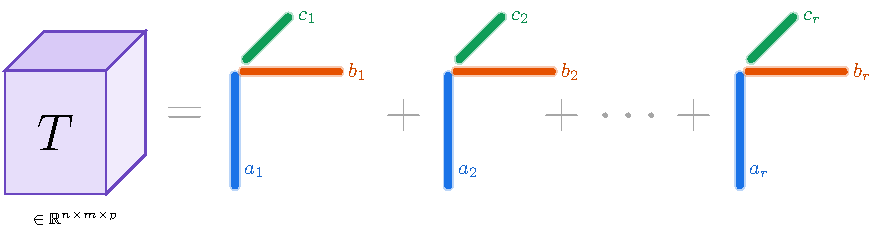
\includegraphics[width=\textwidth, keepaspectratio]{Sources/Chapter1/figures/cp.pdf}
	\caption{Fattorizzazione CP di un tensore $ T = \dsqr{A,B,C} \in \R^{n\times m\times p} $,
		dove i vettori $ a_l,b_l,c_l $ indicano le colonne $ l- $esime di $ A,B,C $.}
	\label{fig:cp_dec}
\end{figure}

\begin{remark}[Risparmio in memoria della CP]
	La fattorizzazione CP di un tensore $ T $ di rango $ r $ permette di ridurre notevolmente il
	costo di memorizzazione, in quanto richiede $ O((n_1 + \ldots + n_d)r) \ll
		O(\prod_{i=1}^d n_j)$.
\end{remark}


\section{Slices, fibers e unfoldings}
\todo{Cambiare}



\begin{definition}[Tensor slice]
	Dato $ T \in \Rmsiz $ chiamiamo \emph{slice (o fetta)} di $ T $ ogni matrice ottenuta da $
		T $ fissando tutti gli indici tranne due. Le slices ottenute fissando gli ultimi $ d-2 $ indici sono dette frontal slices.
	Nel caso $ d=3 $ si identificano tutte le possibili slices (Figura~\ref{fig:tensor_slices}):
	\begin{figure}[htbp]
		\centering
		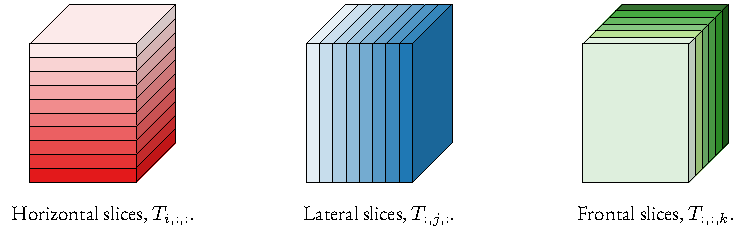
\includegraphics[width=\textwidth, keepaspectratio]{Sources/Chapter1/figures/slices.pdf}
		\caption{Slices di un tensore di ordine 3: fette orizzontali $X_{i::}$ (mode-1), laterali $X_{:j:}$ (mode-2) e frontali $X_{::k}$ (mode-3).}
		\label{fig:tensor_slices}
	\end{figure}
\end{definition}

\begin{definition}[Mode-$k$ fiber]
	Dato un tensore $ T \in \Rmsiz!$ chiamiamo \emph{fibers} i vettori ottenuti fissando
	tutti gli indici tranne uno. Quando l'indice libero di variare è il $ k $-esimo lo chiamiamo
	\emph{mode-$k$ fiber}. Nel caso $ d=3 $ denotiamo le fibre come fibre colonna $x_{:jk}$ (mode-1), fibre riga $x_{i:k}$ (mode-2) e fibre tubo $x_{ij:}$ (mode-3), come illustrato in Figura~\ref{fig:tensor_fibers}.
	\begin{figure}[htbp]
		\centering
		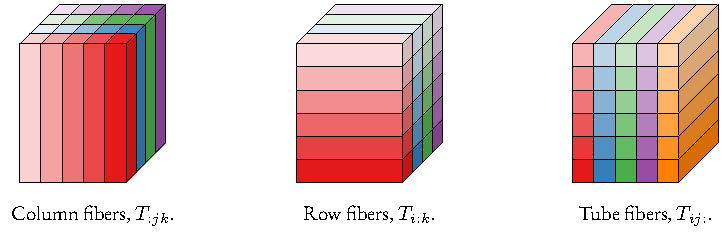
\includegraphics[width=\textwidth, keepaspectratio]{Sources/Chapter1/figures/fibers.pdf}
		\caption{Fibre di un tensore di ordine 3: fibre colonna $x_{:jk}$ (mode-1), riga $x_{i:k}$ (mode-2) e tubo $x_{ij:}$ (mode-3).}
		\label{fig:tensor_fibers}
	\end{figure}
\end{definition}

In molte situazioni risulta comodo disporre gli elementi di un tensore in una matrice. Uno dei modi
per farlo è utilizzare le matricizzazioni, anche dette \emph{unfoldings}.

\begin{definition}[Mode-$k$ unfolding]
	Il \emph{mode-$k$ unfolding} di un tensore $ T \in \Rmsiz! $ è la matrice $ \Tm{T}{k} \in \R^{n_k \times
			\prod_{j\neq k}n_j} $ le cui colonne sono mode-$ k $ fibers ordinate seguendo l'ordine naturale
	su $ \sdom $. In particolare si ha
	\[
		(\Tm{T}{k})_{i,j} = T_{\siwc{i}} \text{, con } j = \L(\siwc)
		.\]
\end{definition}
\begin{remark}
	Possiamo pensare all'unfolding nel modo $ k $ come a rimappare l'indice $ i_{k} $ sulle righe e
	l'indice $ (i_1, \ldots, i_{k-1}, i_{k+1}, \ldots, i_{d}) $ sulle colonne.
\end{remark}

\begin{figure}[htbp]
	\centering
	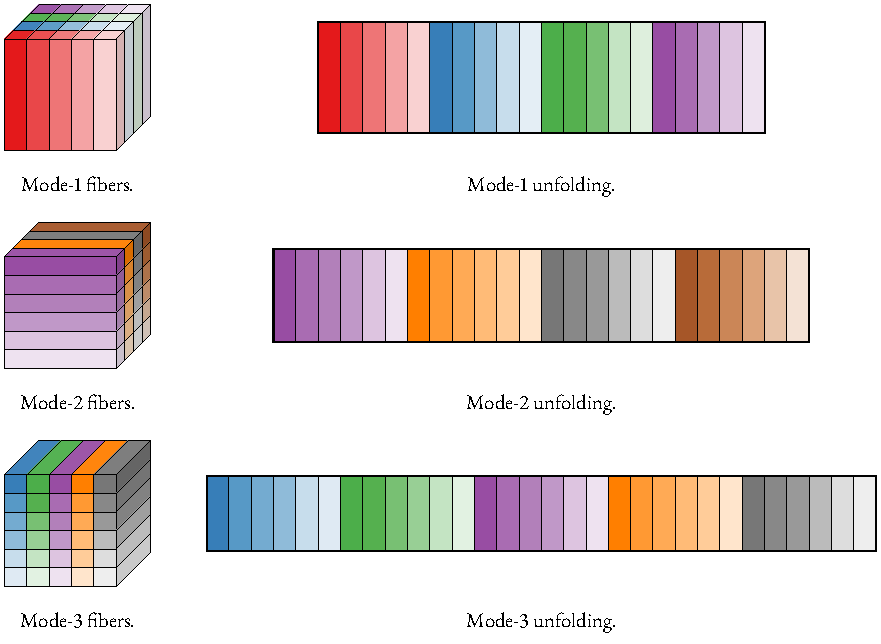
\includegraphics[width=\textwidth, keepaspectratio]{Sources/Chapter1/figures/fibers_unfolding.pdf}
	\caption{Fibre e matricizzazioni nei tre modi per un tensore del terzo ordine.}
	\label{fig:fibers_unfolding}
\end{figure}

\begin{example}[De Lathauwer~\cite{lieven2006}]
	Consideriamo il tensore $ T $ di taglia $ 2\times 2\times 2 $ definito da
	\begin{equation*}
		a_{111}=-a_{121} = 3, \quad a_{211} = -a_{221} = 6, \quad a_{112} = -a_{122} = 1, \quad a_{212} = - a_{222} = 2.
	\end{equation*}
	I vettori dei modi $ 1,2 $ e $ 3 $ sono le colonne delle matrici
	\begin{equation*}
		\Tm{T}{1} = \begin{bmatrix} 3 & -3 & 1 & -1 \\ 6 & -6 & 2 & -2 \end{bmatrix}, \quad
		\Tm{T}{2} = \begin{bmatrix} 3 & 6 & 1 & 2 \\ -3 & -6 & -1 & -2 \end{bmatrix}, \quad
		\Tm{T}{3} = \begin{bmatrix} 3 & 6 & -3 & -6 \\ 1 & 2 & -1 & -2 \end{bmatrix},
	\end{equation*}
	rispettivamente. Il tensore ha rango uno perché si può decomporre come
	\begin{equation*}
		T = \begin{bmatrix} 1 \\ 2 \end{bmatrix}  \topp \begin{bmatrix} 1 \\ -1 \end{bmatrix} \topp
		\begin{bmatrix} 3 \\ 1 \end{bmatrix}.
	\end{equation*}
	Pensando la terza dimensione nel verso entrante al foglio, possiamo riassumere i passaggi svolti
	per fattorizzare $ T $, dove è stata applicata più volte la definizione di prodotto tensore:
	\todo{c'è un typo!}
	\begin{center}
		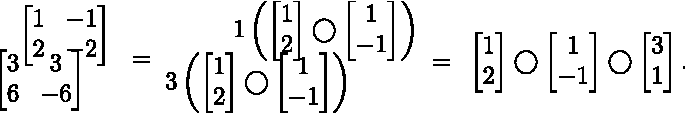
\includegraphics[width=0.65\textwidth, keepaspectratio]{./Sources/Chapter1/figures/cp_example.pdf}
	\end{center}
\end{example}

\begin{figure}[htbp]
	\centering
	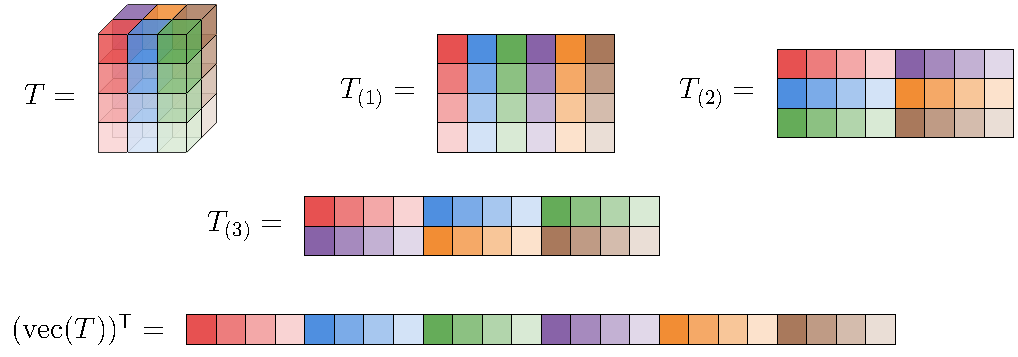
\includegraphics[width=\textwidth, keepaspectratio]{Sources/Chapter1/figures/unfoldings.pdf}
	\caption{Schema delle matricizzazioni e vettorizzazione di un tensore.}
	\label{fig:unfoldings}
\end{figure}
L'operazione di unfolding permette anche di catturare il suo rango (matriciale) lungo ogni direzione:

\todo{anche def landsberg}
\begin{definition}[Rango multilineare]
	Il \emph{rango multilineare} o \emph{multirank} di un tensore $ T \in \Rmsiz $ è la $ d $-upla $
		(r_1, r_2, \ldots, r_d) $, dove $ r_k = \rank{\Tm{T}{k}} $, per ogni $ k \in \{1, \ldots, d\}
	$. Lo denotiamo con $ \multirk(T) $.
\end{definition}


Dal punto di vista computazionale è utile introdurre la seguente operazione

\todo{refrasare un poco per renderla più leggibile}
\begin{definition}[Reshape]
	Definiamo l'operatore di \emph{reshape} come l'operazione riarrangia il tensore senza alterarne le dimensioni e mantenendo l'ordine delle entrate. Formalmente,
	fissati $ d, d' \in \N$ e un tensore $ T \in \Rmsiz! $, per ogni $ m_1, \ldots, m_{d'} $ tali
	che $ \prod_{i=1}^{d'} m_j = \prod_{j = 1}^{d} n_j$, il tensore $ \Tn{y} = \reshape(T,
		\msiz![m][d']) \in \Rmsiz![m][d'] $ è definito come
	\[
		\Tn{y}(i_1, \ldots, i_{d'})= T(j_1, \ldots, j_d)
		,\]
	per ogni $(i_1, \ldots, i_{d'}),(j_1, \ldots,
		j_d) $ tali che $ \L(i_1, \ldots, i_{d'}; \msiz![m][d'])) = \L(j_1, \ldots,
		j_d; \msiz!)$.
\end{definition}
\begin{remark}
	Un reshape ha costo nullo perché non si spostano celle di memoria, ma si eseguono solo operazioni
	di indici. Questa proprietà vale in particolare per tutte le strutture dati (vettori, matrici,
	tensori) $ \tilde{T} $ tali che $ \vec(\tilde{T}) = \vec(T) $.
\end{remark}
\begin{remark}
	L'unfolding sul primo modo ha costo nullo, in quanto $ \Tm{T}{1} = \reshape(T, n_1 \times
		\prod_{j=2}^d n_{j}) $, cioè
	\begin{equation*}
		\Tm{T}{1} = \left[\begin{array}{c|c|c}
				T_{:, \ldots, :,1} & \dots & T_{:, \ldots, :, n_{d}}
			\end{array}\right] \in \R^{n_1 \times
			\prod_{j=2}^d n_{j}}.
	\end{equation*}
\end{remark}
\begin{remark}
	Per $ k>1 $, formare l'unfolding $ \Tm{T}{k} $ ha un costo non banale, in particolare $
		\vec(\Tm{T}{k}) \neq \vec(T) $.

	Se $ k=d $, l'unfolding $ \Tm{T}{d} = \begin{bmatrix} \vec(T_{:, \ldots, :, 1})^{\top} \\  \vdots
			\\ \vec(T_{:, \ldots, :, n_{d}})^{\top}\end{bmatrix}  $, e in particolare vale $
		\vec(\Tm{T}{d}^{\top}) = \vec(T)$. Quindi calcolare la trasposta dell'ultimo unfolding
	non costa nulla.
\end{remark}

\begin{lemma}[Vettorizzazione e unfolding di un tensore di rango uno]
	\label{lhm:vec_unf_rk1}
	Dato un tensore $ T = v^1 \topp \cdots \topp v^d $, allora
	\begin{enumerate}[label=(\roman*)]
		\item $\Vec(T) = v^d \krn \cdots \krn v^1$.
		\item $ \Tm{T}{k} = v^k\left( v^d \krn \cdots \krn v^{k-1} \krn v^{k+1} \krn \cdots
			      \krn v^1 \right)^{\top}$.
	\end{enumerate}
	In particolare, tutte le matricizzazioni di un prodotto esterno hanno rango 1.
\end{lemma}
\begin{proof}
	La $ (i) $ segue applicando più volte l'Osservazione~\ref{rmk:krn_tensor}. Dimostriamo la $ (ii)
	$. Per definizione di tensore di rango uno~\eqref{eq:rk1_components} la scrittura in componenti di $ T $ è
	\begin{equation*}
		T_{i_1, \ldots, i_{d}} = v^1_{i_1} \cdots v^d_{i_{d}} = v^k_{i_{k}} \left( \prod_{\substack{m=1
				\\ m\neq k}}^d v^m_{i_{m}}\right).
	\end{equation*}
	Preso $ u = v^d \krn \cdots \krn v^{k+1} \krn v^{k-1} \krn \cdots \krn v^1 $, osserviamo che la
	sua componente $ j $-esima è il prodotto fra parentesi, ovvero $ u_{j} =\left( \prod_{\substack{m=1
				\\ m\neq k}}^d v^m_{i_{m}}\right) $. A questo punto, per definizione di unfolding abbiamo
	$ \left( \Tm{T}{k} \right)_{i_{k},j} = v^k_{i_{k}}u_{j}$, da cui
	\begin{equation*}
		\Tm{T}{k} = v^k u^{\top} = v^k \left( v^d \krn \cdots \krn v^{k+1} \krn v^{k-1} \krn \cdots \krn
		v^1 \right)^{\top}.
	\end{equation*}
\end{proof}

In molte situazioni è utile moltiplicare un tensore con una matrice, ma purtroppo le dimensioni non
combaciano. La seguente definizione risolve
il problema facendo agire la matrice la matrice lungo il modo $ k- $esimo di un tensore, e si
chiama.
\begin{definition}[Prodotto nel modo $k$]
	Il \emph{prodotto nel modo $ k $} di un tensore $ T \in \Rmsiz! $ con una matrice $ U \in
		\R^{r \times n_k} $ descrive l'azione di $ U $ sulla $ k $-esima coordinata di $ T $. Formalmente, è un tensore
	\[
		Y = T \ttm U \in \R^{\ssiz{r}} \text{ con } \Tm{Y}{k} = U \Tm{T}{k}
		.\]
	In componenti, $ Y_{\siwc{\alpha}} = \sum_{i_k = 1}^d T(\miwc) U_{\alpha, i_k} $.
\end{definition}


\todo{Esempio polinomio semisep + altro es}


\section{Il problema del rango}
\label{sec:cp_rank}

In più dimensioni il problema di calcolare il rango, e una fattorizzazione CP di un tensore si
complicano notevolmente rispetto al caso matriciale.\todo{non mi piace}
Ci sono molte domande aperte riguardo al rango, ad esempio non si ha una risposta generale (a
differenza del
caso matriciale) a domande del tipo:
\begin{enumerate}
	\item Qual'è il massimo rango possibile per un tensore di dimensione $ n_1 \times \cdots \times n_d $?
	\item Quali sono i ranghi \emph{tipici}, ovvero quelli ottenuti con probabilità non nulla quando si genera un tensore di entrate casuali?
\end{enumerate}
Per capire il motivo, discutiamo alcune caratteristiche dei tensori che rendono complesso il ``problema del
rango''.

\subsection*{Border rank}
Nel caso delle matrici, una successione di matrici di rango $ r $ converge sempre a una matrice di
rango $ \le r $. Per i tensori possono accadere dei ``salti'', in altre parole, la varietà dei
tensori di un rango fissato $ r $ non è chiusa\footnote{Non precisiamo la topologia, per una
	discussione formale si vedano~\cite{landsberg2011tensors,landsberg2015geometry}.}, ad esempio, un tensore di rango $ 2 $
può convergere ad uno di rango $ 3 $, come mostra il prossimo esempio. Questo inconveniente teorico
ha risvolti interessanti che vedremo nella \S~\ref{sec:APA}.

\begin{example}
	\label{ex:border_rank}
	Consideriamo dei vettori $ a_1,a_2 \in \R^m$, $b_1,b_2 \in \R^n$ e $c_1,c_2\in \R^p $ vettori
	linearmente indipendenti. Definiamo il tensore
	\begin{equation}
		T = a_1 \topp  b_1 \topp c_2 + a_1 \topp b_2 \topp c_1 + a_2 \topp b_1 \topp c_1,
	\end{equation}
	e notiamo che $ \rk(T) = 3 $ dato che non può
	essere scomposto come somma di tensori più semplici.
	Consideriamo la successioni di tensori
	\begin{equation}
		\label{eq:rank_counterex}
		T_\varepsilon = \frac{1}{\varepsilon}\left( a_1 +
		\varepsilon a_2 \right) \topp (b_1 + \varepsilon b_2) \topp (c_1 + \varepsilon c_2) -
		\frac{1}{\varepsilon} a_1 \topp b_1 \topp c_1, \text{ con } \varepsilon \in \R,
	\end{equation}
	che essendo combinazione lineare di due tensori di rango uno, ha rango 2.
	Vediamo che $ \lim_{\varepsilon \to 0} T_\varepsilon = T $, da cui segue che l'insieme dei tensori di rango 3 non è chiuso.
	Espandendo i termini dell'Equazione \eqref{eq:rank_counterex} tramite la proprietà distributiva del prodotto esterno,
	\begin{equation}
		\begin{aligned}
			\Tn{y}_\varepsilon & =  \frac{1}{\varepsilon} a_1 \topp b_1 \topp c_2 + a_1 \topp b_1 \topp c_2 + a_1 \topp b_2 \topp c_1
			+a_2 \topp b_1 \topp c_1                                                                                                  \\ &+ \varepsilon \left(a_2 \topp b_2 \topp c_1 + a_1 \topp b_1 \topp c_2 +
			a_1 \topp b_2 \topp c_2 + a_2 \topp b_2 \topp c_2 \right) - \frac{1}{\varepsilon} a_1 \topp
			b_1 \topp c_1                                                                                                             \\
			                   & = T + \varepsilon\left(a_2 \topp b_2 \topp c_1 + a_1 \topp b_1 \topp c_2 +
			a_1 \topp b_2 \topp c_2 + a_2 \topp b_2 \topp c_2 \right)
		\end{aligned}
	\end{equation}
	Quindi $ T_\varepsilon - T \to 0 $.
\end{example}

Questo motiva la seguente definizione:


\begin{definition}[Border rank]
	Un tensore $ T $ ha \emph{border rank} $ r $ se è limite di una successione di tensori di
	rango $ r $, ma non è limite di una successione di tesori di rango $ s $, per ogni $ s < r $. Lo
	denoteremo con il simbolo $ \brk(T) $.
\end{definition}
\begin{remark}
	$ \rk(T) \ge \brk(T) $.
\end{remark}
\begin{remark}
	In altri termini, se $ T \in \Rmsiz $, il suo border rank è la quantità
	\[
		\brk(T) = \min \left\{ r \in \N \mid \exists T' \in \Rmsiz! \text{ tale che }
		\rk(T')=r, \, \|T - T'\|  < \varepsilon \right\}
		.\]
\end{remark}
\todo{Disegno interpretazione geometrica (landsberg pg 38)}

Il border rank ammette anche la seguente interpretazione geometrica:




\subsection*{Costo computazionale}
\label{sec:computing_rank}
Calcolare il costo di una fattorizzazione CP usando un algoritmo esatto è NP-Hard~\cite{haastad1989tensor}. Non
solo; il problema di trovare un tensore approssimante di un certo rango è computazionalmente
difficile. In altre parole, la miglior approssimazione di rango $ r $ è data da dei vettori $ x_{i}
	\in \R^{n_1}, y_{i} \in \R^{n_2}, \ldots, z_{i} \in \R^{n_{d}}   $, per $ i = 1, \ldots, r $ che minimizzano
\begin{equation*}
	\| A - x_1 \otimes y_1 \otimes \cdots \otimes z_1 - \cdots x_{r} \otimes y_{r} \otimes \cdots
	\otimes z_{r}\|
\end{equation*}
oppure, in altre parole un tensore $ B $ dato da una fattorizzazione CP, che realizza
\begin{equation*}
	\min_{\rank(B) \le r} \| A - B \|.
\end{equation*}
Qui $ \| \cdot \| $ denota una norma fissata su $ \R^{n_1 \times  \cdots \times n_{d}}$. Quando $ d =2$, il
problema è risolto per norme invarianti per trasformazioni unitarie su $ \R^{m \times n} $ dal
teorema di Eckart-Young-Mirsky~\cite{eckart1936approximation}: se
\begin{equation*}
	A = U\Sigma V^* = \sum_{i = 1}^{\rank(A)}\sigma_i u_{i} \otimes v_{i}, \qquad \sigma_{i} \ge
	\sigma_{i+1},
\end{equation*}
è la decomposizione ai valori singolari di $ A $ (anche detta SVD), allora la migliore
approssimazione di rango $ r $ è data dai primi $ r $ termini della somma.
Sfortunatamente, generalizzare questo risultato in più dimensioni è
ritenuto molto difficile (o impossibile)~\cite{desilva2008tensorrankillposednessbest}.

Nella pratica esistono diverse euristiche per calcolare il rango. Una di queste è scegliere come rango il più piccolo $ r $ che minimizza l'errore
relativo rispetto al rango $ r-1 $. Per un tensore a $ 3 $ indici, l'\emph{errore relativo} è
definito in questo modo:
\begin{equation}
	\label{eq:rel_error}
	\varepsilon_{\text{rel}} = \frac{\| T - \dsqr{A,B,C} \|}{\|T\|} = \frac{\left(\sum_{i,j,k}\left( t_{ijk} -
		\sum_{l=1}^r a_{il}b_{jl}c_{kl}\right)^2 \right)^{\frac{1}{2}}}{\left( \sum_{i,j,k}
		t_{ijk}
		\right)^{\frac{1}{2}}}.
\end{equation}

\subsection*{Rango massimo}

Nel caso di una matrice $ m \times n $, il suo rango massimo è $ \min \{m,n\}  $. Per un tensore, il
\emph{rango massimo} è definito come il massimo dei ranghi realizzabili per dei tensori $ T \in
	\R^{n_1 \times \cdots \times n_{d}} $ di una certa taglia fissata. In altre parole,
\begin{equation*}
	\rk_{\text{max}}(\R^{n_1\times n_2 \times \cdots \times  n_{d}}) = \max \{ \rk(T) \mid T \in
	\R^{n_1 \times n_2 \times \cdots \times n_{d}}\}.
\end{equation*}
Sfortunatamente, ad eccezione di alcuni casi speciali, i ranghi massimi per la maggior parte dei
tensori di ordine superiore sono sconosciuti. I casi speciali in cui il rango massimo è noto sono elencati nella Tabella~\ref{tab:max_ranks}. Il primo risultato per tensori di dimensione $2 \times m \times n$ implica, ad esempio, che un tensore di taglia $2 \times 2 \times 2$ ha un rango massimo pari a $3$.

\begin{table}[htbp]
	\centering
	\small
	\caption{Ranghi massimi tensoriali noti. L'ordine delle dimensioni non modifica il rango, quindi le taglie sono ordinate dalla più piccola alla più grande (tratta da Ballard e Kolda~\cite[Tabella~16.1]{BK25}).}
	\label{tab:max_ranks}
	\begin{tabular}{lll}
		\toprule
		Taglia tensore                     & Rango massimo                           & Fonte                                            \\
		\midrule
		$2 \times m \times n \; (m \le n)$ & $m + \min \{ m, \lfloor n/2 \rfloor \}$ & JáJá~\cite{jaja1979}; Kruskal~\cite{kruskal1989} \\
		$3 \times 3 \times 3$              & $5$                                     & Kruskal~\cite{kruskal1989}                       \\
		$3 \times 7 \times 7$              & $8$                                     & Atkinson e Stephens~\cite{atkinson1979}          \\
		$2 \times 4 \times 4$              & $6$                                     & ten Berge~\cite{tenberge2000b}                   \\
		\bottomrule
	\end{tabular}
\end{table}

È inoltre possibile derivare un limite superiore debole per il rango massimo:
\todo{se lasci verificalo}
\begin{equation}
	\label{eq:weak_upper_bound_max_rank}
	\rk_{\text{max}}(\R^{n_1 \times n_2 \times \cdots \times n_d}) \le \min_k \prod_{\substack{\ell=1 \\ \ell \neq k}}^d n_\ell = \frac{\prod_{k=1}^d n_k}{\max_k n_k}.
\end{equation}



\subsection*{Rango tipico}
\label{sec:rango_tipico}

Mentre le matrici random hanno rango massimo con probabilità uno\footnote{L'idea è presa una matrice
	con entrate estratte da una distribuzione di probabilità continua, il
	determinante è un polinomio le cui indeterminate sono le entrate della matrice. Il luogo di
	zeri di questo polinomio ha misura di Lebesgue nulla, quindi integrando la densità di probabilità
	sul luogo di zeri dà probabilità nulla. La tesi si ha passando al compolementare.}, per un tensore di un
formato fissato potrebbe esserci più di un rango con probabilità positiva. Questo fenomeno è noto
come \emph{rango tipico}.

Sia $ \mathcal{D}(n_1, n_2, \ldots, n_{d})$ una distribuzione di probabilità continua sullo spazio
dei tensori $ \R^{n_1 \times n_2 \times \cdots \times n_{d}} $ (un esempio sono i tensori a entrate
gaussiane).
\begin{definition}
	Il \emph{rango tipico} (o \emph{rango generico}) di un tensore $ T \in \K^{n_1 \times \cdots
			\times n_{d}} $ è l'insieme dei ranghi che occorrono con probabilità non nulla, rispetto ad
	ogni distribuzione continua $  \mathcal{D}(n_1, n_2, \ldots, n_{d})$ sull'insieme di tali tensori.
	In formule,
	\begin{equation*}
		\rk_{\text{typical}} = \{r \mid P \left( \rk(T) = r, \; T \sim \mathcal{D}(n_1, \ldots,
			n_{d})\right) > 0\}.
	\end{equation*}
\end{definition}

\todo{rewrite and verify}

Mentre per le matrici il rango tipico è unico e coincide con il massimo rango possibile, per i
tensori di ordine superiore a due. In particolare su $\mathbb{R}$ possono coesistere
più ranghi tipici, mentre su $\mathbb{C}$ il rango tipico è sempre unico. La Tabella~\ref{tab:typical_ranks} riassume i principali risultati noti in letteratura, tratti da Ballard e Kolda~\cite[p.~276, Tabella~16.2]{BK25}.
Per verificare questi risultati, abbiamo implementato un esperimento numerico.
Selezionando alcuni formati, abbiamo generato dei tensori casuali con entrate estratte
indipendentemente sia da una distribuzione normale standard $\mathcal{N}(0, 1)$ sia da una
distribuzione uniforme $\mathcal{U}(-1, 1)$. Il rango di ciascun tensore è stato stimato
usando l'algoritmo ALS\todo{ref} su un campione di $ 200 $ tensori, facendo $ 120 $ restarts e un
numero massimo di $ 500 $ iterazioni, interrompendo una volta raggiunto un errore relativo inferiore a
$10^{-5}$. La distribuzione empirica dei ranghi riportata in Figura~\ref{fig:typical_ranks_dist} mostra che la
distribuzione delle entrate (normale o uniforme) non altera l'insieme dei ranghi tipici e produce frequenze empiriche analoghe.

\begin{figure}[htbp]
	\centering
	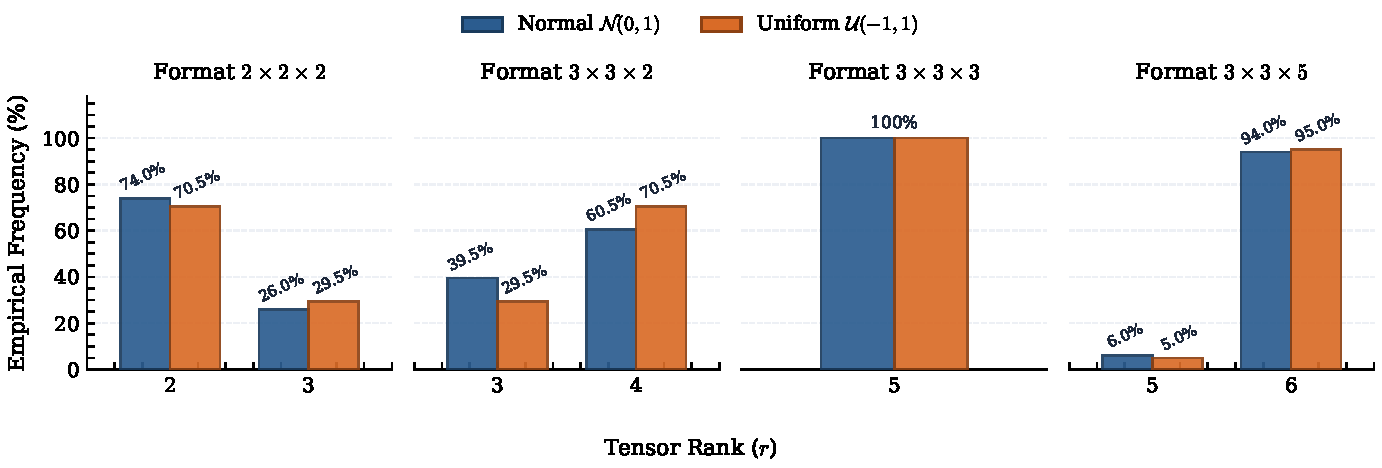
\includegraphics[width=\textwidth, keepaspectratio]{Sources/Chapter1/figures/typical_rank_distribution.pdf}
	\caption{Distribuzione empirica dei ranghi per tensori casuali reali di formato $2 \times 2 \times 2$, $3 \times 3 \times 2$, $3 \times 3 \times 3$ e $3 \times 3 \times 5$ con entrate estratte da distribuzioni Normali $\mathcal{N}(0, 1)$ ed Uniformi $\mathcal{U}(-1, 1)$ (istogrammi affiancati).}
	\label{fig:typical_ranks_dist}
\end{figure}

\begin{table}[htbp]
	\centering
	\small
	\caption{Ranghi tipici noti sul campo reale $\mathbb{R}$ per tensori di dimensione $m \times n \times p$ con $2 \le m \le n \le p$ (adattata da Ballard e Kolda~\cite[Tabella~16.2]{BK25}).}
	\label{tab:typical_ranks}
	\begin{tabular}{lll}
		\toprule
		Formato ($m \times n \times p$)                   & Rango tipico & Fonte                                                                \\
		\midrule
		$2 \times n \times n$                             & $\{n, n+1\}$ & ten Berge, Kiers~\cite{tenberge1999}                                 \\
		$3 \times 3 \times 3$                             & $5$          & ten Berge, Stegeman~\cite{tenberge2006}                              \\
		$3 \times 3 \times 5$                             & $\{5, 6\}$   & ten Berge, Sidiropoulos, Rocci~\cite{tenberge2004}                   \\
		$3 \times 4 \times 8$                             & $\{8, 9\}$   & Sumi et al.~\cite{sumi2013}                                          \\
		$3 \times 5 \times 9$                             & $\{9, 10\}$  & Choulakian~\cite{choulakian2010}; ten Berge~\cite{tenberge2011}      \\
		$4 \times 4 \times 12$                            & $\{12, 13\}$ & Friedland~\cite{friedland2012}                                       \\
		$m \times n \times n(m-1)$ ($m > 2$, $n$ dispari) & $n(m-1)$     & ten Berge~\cite{tenberge2000b}                                       \\
		$m \times n \times p$ ($n(m-1) < p < mn$)         & $p$          & ten Berge, Kiers~\cite{tenberge1999}; ten Berge~\cite{tenberge2000b} \\
		$m \times n \times p$ ($p \ge mn$)                & $mn$         & ten Berge, Kiers~\cite{tenberge1999}; ten
		Berge~\cite{tenberge2000b}                                                                                                              \\
		\bottomrule
	\end{tabular}
\end{table}


\subsection*{Dipendenza dal campo base}
Nel caso matriciale ogni matrice $ m \times n $ a entrate reali ha lo stesso
rango se visto come elemento di $ \R^{m\times n} $ o di $ \C^{m \times n} $, per i tensori questo è
falso. Consideriamo il seguente esempio:
\begin{example}[De Silva e Lim~\cite{desilva2008tensorrankillposednessbest}]
	Scriviamo $ z_{k} = x_{k} + \I y_{k} $ e $ \overline{z}_k = x_{k} - \I y_{k} $, allora
	\begin{equation}
		\begin{aligned}
			 & \frac{1}{2}\left( \overline{z}_1 \topp z_2 \topp \overline{z}_3 + z_1 \topp \overline{z}_2 \topp
			z_3\right)                                                                                          \\
			 & = x_1 \topp x_2 \topp x_3 + x_1 \topp y_2 \topp y_3 - y_1 \topp x_2 \topp
			y_3 + y_1 \topp y_2 \topp x_3.
		\end{aligned}
	\end{equation}
	Chiamando $ I = \overline{z}_{1} \otimes z_2 \otimes \overline{z}_3 $ e $ II = z_1 \otimes
		\overline{z}_{2} \otimes z_3 $, usando la proprietà distributiva e la trilinearità del prodotto
	tensore,
	\begin{equation*}
		\begin{aligned}
			I  & = (x_1 - \I y_1) \otimes (x_2 + \I y_2) \otimes (x_3 - \I y_3)                              \\
			   & = x_1 \otimes x_2 \otimes x_3 - \I x_1 \otimes x_2 \otimes y_3 + \I x_1 \otimes y_2 \otimes
			x_3                                                                                              \\
			   & + x_1 \otimes y_2 \otimes y_3 - \I y_1 \otimes x_2 \otimes x_3 - y_1 \otimes x_2 \otimes
			y_3                                                                                              \\
			   & + y_1 \otimes y_2 \otimes x_3 - \I y_1 \otimes y_2 \otimes y_3,                             \\
			II & = (x_1 + \I y_1) \otimes (x_2 - \I y_2) \otimes (x_3 + \I y_3)                              \\
			   & =x_1 \otimes x_2 \otimes x_3 + \I x_1 \otimes x_2 \otimes y_3 - \I x_1 \otimes y_2
			\otimes x_3                                                                                      \\
			   & + x_1 \otimes y_2 \otimes y_3 + \I y_1 \otimes x_2 \otimes x_3 - y_1 \otimes x_2 \otimes
			y_3                                                                                              \\
			   & + y_1 \otimes y_2 \otimes x_3 + \I y_1 \otimes y_2 \otimes y_3.
		\end{aligned}
	\end{equation*}
	L'espressione sopra segue calcolando $ \frac{1}{2}(I + II) $.

\end{example}

\section{Il teorema del rango}

Data la complessità del problema del rango possiamo stimarlo rango con la seguente
proposizione, dalla quale intuiamo che non sarà semplice trovare stime del rango di un
tensore---queste spesso coinvolgono tecniche algebrico-combinatoriche avanzate. Vedremo alcuni esempi di
queste stime nella Sezione~\ref{sec:exp_estimates}.

Definiamo un'operazione utile tra le colonne di due matrici, che sarà utile a dimostrare il
risultato di questa sezione.
\begin{definition}[Prodotto Khatri-Rao]
	Date due matrici $ A \in \R^{m \times r} $ e $ B \in \R^{n \times r} $, il loro \emph{prodotto
		Khatri-Rao} è dato da
	\begin{equation}
		C = A \krp B = \left[ a_1 \krn b_1 \mid \ldots \mid a_r \krn b_r \right] \in \R^{(mn) \times r},
	\end{equation}
	dove $ a_j $ e $ b_j $ indicano la $ j$-esima colonna di $ A $ e $ B $, rispettivamente, e la matrice $ C $
	si lascia scrivere in componenti come $ C_{kl} = A_{il}B_{jl} $, dove $ \L^*(i,j) = \L(j,i) = k $.
\end{definition}
\begin{remark}
	\label{rmk:krp_sub_krn}
	Il prodotto $ A \krp B $ è sottomatrice di $ A \krn B $, in quanto una colonna $ k $-esima della
	prima è del tipo $ a_{k} \krn b_{k} $, mentre per la seconda è $ \left[ a_{1k}B, \ldots, a_{mk}B
			\right]^{\top} $; quindi possiamo ottenere la prima matrice selezionando alcune colonne della
	seconda.
\end{remark}
\begin{remark}
	\label{rmk:krp_as_span}
	Data una fattorizzazione $ T = \dsqr{U_1, \ldots, U_{d}}$, il prodotto Khatri-Rao
	\begin{equation*}
		U_{d} \krp U_{d-1} \krp \cdots \krp U_1
	\end{equation*}
	ha come colonna $ r $-esima $ u^d_r \krn u^{d-1}_r \krn \cdots  \krn u^1_r$, in altre parole, è la
	rappresentazione matriciale dell'insieme $ \left\{ u^d_r \krn u^{d-1}_r \krn \cdots  \krn u^1_r\right\}_{r=1,
				\ldots, d} $ formato
	dagli addendi della decomposizione $ \vec(T) = \sum_{r=1}^R u^d_r \krn u^{d-1}_r \krn \cdots  \krn u^1_r $.
	In particolare, vale
	\begin{equation*}
		\begin{aligned}
			\Vec({T}) & = \sum_{h=1}^r u_h^d \krn \cdots \krn u_h^1 = \left[ u_1^d
			\krn \cdots \krn u_1^1 | \cdots | u_r^d \krn \cdots \krn u_r^1\right]^{\top}\mathbf{1}_r \\
			          & = \left( U_d \krp U_{d-1} \krp \cdots \krp U_1 \right) \mathbf{1}_r.
		\end{aligned}
	\end{equation*}

\end{remark}

\begin{remark}
	Calcolare il prodotto di Khatri-Rao di due matrici $ A \in \R^{m \times r} $ e $ B \in \R^{n \times
			r} $ ha un costo in memoria di $ O(mn
		r) $.
\end{remark}

\begin{lemma}
	\label{lhm:krp_unfoldings}
	Data una fattorizzazione $ T = \dsqr{U_1,\ldots, U_d} \in \Rmsiz!$, essa ha come unfoldings
	\[
		\Tm{T}{j} = U_j \left( U_d \krp U_{d-1} \cdots \krp U_{j+1} \krp U_{j-1} \krp \cdots U_1 \right)^{\top}
		,\]  per ogni $ j = 1, \ldots, d $.
\end{lemma}
\begin{proof}
	Scrivendo le matricizzazioni di $ T = \sum_{h=1}^r u_h^1 \topp \cdots \topp u_h^d $, dove i vettori $ u_1^j,
		\ldots, u_r^j $ rappresentano le colonne della matrice $ U_j $, troviamo che
	\begin{equation*}
		\begin{aligned}
			\Tm{T}{j} & = \sum_{h=1}^r u_h^j \left( u_h^d \krn \cdots \krn u_h^{j+1} \krn u_h^{j-1} \krn
			\cdots \krn u_h^1 \right)^{\top}                                                             \\
			          & = U_j \begin{bmatrix} u_1^d \krn \cdots \krn u_1^1 | \cdots | u_r^d \krn \cdots
				                  \krn u_r^1\end{bmatrix}^{\top}   \\
			          & = U_j \left( U_d \krp \cdots \krp U_{j+1} \krp U_{j-1} \krp \cdots \krp U_1
			\right)^{\top},
		\end{aligned}
	\end{equation*}
	dove nel primo passaggio abbiamo applicato la Proposizione~\ref{lhm:vec_unf_rk1} su ogni addendo di rango uno.
\end{proof}
\begin{example}
	Se $ T = \dsqr{A,B,C} $, allora segue che $ \Tm{T}{1} = A \left( C \krp B \right)^{\top} $.
\end{example}




\begin{proposition}[Teorema del rango]
	\label{th:rank}
	Sia $ T \in \Rmsiz! $ un tensore che ammette fattorizzazione $ T = \dsqr{U_1, \ldots,
			U_d} $, e sia $ r_j = \rank(\Tm{T}{j}) $ il rango dell'unfolding $ \Tm{T}{j} $ con $ j = 1, \ldots, d $. Allora vale che
	\begin{equation}
		\max_{j=1, \ldots, d}(r_j) \le \rk(T) \le \min_{j=1, \ldots, d}\left( \prod_{i \neq j}r_i \right)
	\end{equation}
\end{proposition}
\begin{proof}
	Fissato $ r = \rk(T) $, la minorazione segue direttamente dal fatto che ogni unfolding $ \Tm{T}{j}
	$ è una matrice di taglia $ n_{j} \times r  $.
	Mostriamo la maggiorazione, assumendo senza perdita di generalità che $ \rk(T) \le
		\prod_{i=2}^d r_i $. Consideriamo la vettorizzazione
	\begin{equation}
		\label{eq:vec_rk_krn}
		\Vec(T) = \sum_{k=1}^r u_k^d \krn \cdots \krn u_k^2 \krn u_k^1.
	\end{equation}
	Allora l'insieme
	\[
		\left\{u_k^d \krn \cdots \krn u_k^2\right\}_{k = 1, \ldots, r}
	\] è formato da vettori linearmente indipendenti. Se così non fosse,
	esisterebbe un indice $ k_0 $, che possiamo supporre $ k_0 = 1 $ a meno di riordinamento degli
	indici $ k $, tale per cui
	\begin{equation}
		u_{1}^d \krn \cdots \krn u_{1}^2 = \sum_{h = 2}^r c_h(u_h^d \krn \cdots \krn u_h^2),
	\end{equation}
	che sostituita nella Equazione~\eqref{eq:vec_rk_krn} porta alla seguente decomposizione:
	\begin{equation*}
		\begin{aligned}
			\Vec(T) & = \sum_{k=2}^r u_k^d \krn \cdots \krn u_k^2 \krn u_k^1 + \left(\sum_{k=2}^r c_k
			\left(u_k^d \krn \cdots \krn u_k^2\right) \right) \krn u_1^1                              \\
			        & = \sum_{k=2}^r \left(u_k^d \krn \cdots \krn u_k^2\right)
			\krn \left(u_k^1 + c_k u_1^1\right)
		\end{aligned},
	\end{equation*}
	che ha rango $ r-1 $, contraddicendo la minimalità di $ r $.
	Dal Lemma~\ref{lhm:krp_unfoldings} possiamo scrivere
	\[
		\Tm{T}{1} = U_1 \left( U_d \krp \cdots \krp U_2 \right)^{\top}.
	\] Dalla lineare indipendenza appena dimostrata, e
	dall'Osservazione~\ref{rmk:krp_as_span} segue che $ \rk \left(U_d \krp \cdots \krp U_2 \right) =r $.
	Applicando l'Osservazione~\ref{rmk:krp_sub_krn} a più fattori, $ U_d \krp \cdots \krp U_r $ è
	sottomatrice di $ U_d \krn \cdots \krn U_2 $. Siccome il rango del prodotto di Kroneker è
	moltiplicativo (Osservazione~\ref{rmk:rk_krn_prod}) troviamo
	\begin{equation*}
		r \le \rank \left(U_d \krn \cdots \krn U_2 \right) = r_2 \cdots r_d.
	\end{equation*}
	Ripetendo l'argomento per gli altri unfoldings si ha la tesi.
\end{proof}

\begin{remark}
	Una conseguenza immediata di questo teorema è che $ T $ ha rango uno se e solo se $ \multirk(T) =
		1$, cioè se e solo se $ \rk(\Tm{T}{j}) = 1 $ per ogni $ j $.
	In generale vale che, se $ \rk(T) = r $, allora $ \multirk(T) \le r $, ma non il
	viceversa.\todo{ho cercato un esempio non è semplice verificare}

\end{remark}


\section{Ricostruzione del tensore in formato denso}

In alcune situazioni è utile scrivere il tensore fattorizzato in modo esplicito, ad esempio per
valutare l'errore di approssimazione~\eqref{eq:rel_error} o generare numericamente un tensore. Un modo conveniente
di farlo è il seguente. Data una fattorizzazione $ T = \dsqr{A,B,C} \in \R^{m\times n\times p} $ di
rango $ r $,
dato che $ \vec(T) = \left( C \krp B \krp A \right)\bm{1}_{r} $, saremmo tentati di formare la matrice $ C
	\krp B \krp A $ e moltiplicarla per il vettore di tutti uni $ \bm{1}_{r} $, ma questa matrice ha più
entrate del risultato finale. L'approccio vincente è considerare $ \Tm{T}{1} = A \left( C \krp B
	\right)^{\top} $ dato dalla Proposizione~\ref{lhm:krp_unfoldings}, e studiare il sistema
\begin{equation*}
	\begin{cases}
		R = C \krp B,  \\
		Y = AR^{\top}, \\
		T = \reshape(Y, m \times n\times p).
	\end{cases}
\end{equation*}
Il risultato intermedio $ R \in \R^{np \times r} $ ha costo $ O(npr) $, mentre formare $ Y $ costa $
	O(mnpr) $. Dato che l'unfolding è sul modo uno, non abbiamo bisogno di permutazioni.


\section{Calcolo della fattorizzazione CP}
\label{sec:computing_cp}

Trattiamo il problema di trovare la migliore approssimazione con rango $ r $ di un dato tensore.
Studiamo il caso $ d = 3 $ per semplicità di notazione.
Dato $ T \in \R ^ {m \times n \times p} $ cerchiamo una fattorizzazione $ \dsqr{A, B, C} $ con
$ A \in \R^{m \times r}, B \in \R^{n\times r} $ e $ C \in \R^{p \times r} $ cercando di risolvere il
problema ai minimi quadrati
\begin{equation}
	\tag{$\mathcal{P}$}
	\label{eq:least_square_tensor}
	\min_{A,B,C}\| T - \dsqr{A,B,C}\|^2.
\end{equation}
Tale problema può essere mal posto per quanto detto sul border rank. Inoltre si tratta di un
problema non convesso (esistono molti minimi locali); inoltre un tensore può avere
fattorizzazioni CP multiple.

\begin{definition}[Prodotto di Hadamard]
	Date due matrici $ A,B \in \R^{m\times n} $, il loro \emph{prodotto di Hadamard} è il loro
	prodotto elemento per elemento, e si indica con la matrice $ C = A \had B $ con entrate $ C_{ij} =
		a_{ij}b_{ij} $.
\end{definition}
\begin{lemma}
	\label{lhm:had_krp}
	Date delle matrici $ A \in \R^{m\times r}, B \in \R^{n \times r}, C \in \R^{m\times s}, D \in
		\R^{n\times s} $, vale
	\begin{equation*}
		\left( A \krp B \right)^{\top} \left( C \krp D \right) = (
		A^{\top}C ) \had ( B^{\top}D ).
	\end{equation*}
\end{lemma}
\begin{proof}
	Basta osservare che la matrice
	\todo{array ticker brackets []}
	\begin{equation*}
		\begin{aligned}
			(A \krp B)^{\top}(C \krp D) =
			\begin{bmatrix} a_1^{\top} \krn b_1^{\top} \\ \vdots \\
				a_{r}^{\top} \krn b_{r}^{\top}
			\end{bmatrix} \left[\begin{array}{c|c|c}
					                    c_1 \krn d_{1} & \dots & c_{s} \krn d_{s}
				                    \end{array}\right].
		\end{aligned}
	\end{equation*}
	ha come entrata $ (i,j) $ l'elemento $ (a_{i}^{\top}c_{j})(b_{i}^{\top}d_{j}) $, che corrisponde
	all'entrata $ (i,j) $ di $ (A^{\top}C ) \had ( B^{\top}D ) $.
\end{proof}



\subsubsection{Alternating least-squares}

Nonostante la funzione obbiettivo dell'Equazione~$\eqref{eq:least_square_tensor}$ non sia convessa,
essa è convessa nelle singole variabili. Ovvero, fissando $ B $ e $ C $, ottimizzare solo su $ A $
significa risolvere un problema ai minimi quadrati lineare
\begin{equation}
	\label{eq:lsq_matrix}
	\| T - \dsqr{A,B,C}\|^2 = \| \Tm{T}{1} - A(C \krp B)^{\top}\|_F^2 = \| (C \krp B)A^{\top} -
	\Tm{T}{1}^{\top}\|_F^2,
\end{equation}
dove l'incognita è una matrice. Nel primo
passaggio abbiamo applicato la Proposizione~\ref{lhm:krp_unfoldings} per ridurci a un problema ai
minimi quadrati matriciale.
La soluzione può essere espressa \todo{why?} in termini delle equazioni normali
\[
	(C \krp B)^{\top}(C \krp B)A^T = (C \krp B)^{\top}\Tm{T}{1}^{\top}
	,\]
se e solo se, usando il Lemma~\ref{lhm:had_krp}
\begin{equation}
	\label{eq:als_pseudoinverse_eq}
	(C^{\top}C \had B^{\top}B)A^{\top} = (C \krp B)^{\top}\Tm{T}{1}^{\top}
\end{equation}
Sia $ Z \defeq C^{\top}C \had B^{\top}B \in \R^{r\times r} $. Osserviamo che calcolare $ Z $ ha costo $
	O((n+p)r^2) $. Inoltre $ Z $ è semidefinita positiva\todo{motiva}, e quando $ C
	\krp B$ è full-rank è positiva definita: in tal caso possiamo risolvere con la fattorizzazione di Cholesky il sistema
\begin{equation}
	AZ = \Tm{T}{1}(C\krp B)= M,
\end{equation}
con costo $ O(r^2m + r^3) $ \todo{verifica}

L'idea dell'algoritmo ALS è di minimizzare ciclicamente la funzione obiettivo
dell'Equazione~\eqref{eq:lsq_matrix}, prima al variare di $ A $, poi $ B $ e poi $ C $. Ognuno dei problemi dati dall'Equazione ha costo $
	O(mnpr) $\todo{verificare (aggiungerebbe un paragrafetto)}. Riassumiamo questo schema
nell'Algoritmo~\ref{alg:ALS}, dove in ogni passaggio riscaliamo la fattorizzazione CP come $
	\dsqr{AD_{A}, BD_{B}, CD_{C}} $ con delle
matrici tali che $ D_{A}D_{B}D_{C} = I_{r} $ per riscalare le colonne dei due fattori fissati in
modo che abbiano norma unitaria.

\begin{algorithm}[htbp]
	\caption{Schema dell'algoritmo ALS.}
	\label{alg:ALS}
	\begin{algorithmic}[1]
		\Require Tensore $ T $ di rango $ r $, tolleranza $ \varepsilon $.
		\State Generiamo $ B $ e $ C $ in modo casuale.
		\State Normalizziamo le colonne di $ B $.
		\Repeat
		\State Normalizziamo le colonne di $ C $.
		\State $ A \gets \arg \min_{A} \| T - \dsqr{A,B,C} \|^2 $.
		\State Normalizziamo le colonne di $ A $.
		\State $ B \gets \arg \min_{B} \| T - \dsqr{A,B,C} \|^2 $.
		\State Normalizziamo le colonne di $ B $.
		\State $ C \gets \arg \min_{C} \| T - \dsqr{A,B,C} \|^2 $.
		\Until{$ \frac{\| T - \dsqr{A,B,C} \|}{\|T\|} > \varepsilon $.}
	\end{algorithmic}
\end{algorithm}

\begin{remark}
	Dato che in genere non si sa il valore ottimo del problema~$\eqref{eq:least_square_tensor}$,
	arrestiamo l'algortmo quando sta ``stagnando'', ovvero quando l'errore relativo fra due iterazioni
	successive diminuisce meno di un dato fattore.
\end{remark}

\begin{remark}
	Nel caso di $ T $ matrice, il fattore $ C = I $ e nel caso $ T $ ha rango $ r=1 $, l'algoritmo diventa il
	metodo delle potenze, in quanto l'Equazione~\eqref{eq:als_pseudoinverse_eq} degenera in $ a \gets
		T \frac{b}{\|b\|^2}$ e $ b \gets T^{\top}\frac{a}{\|a\|^2} $, mentre per $ T $ di rango $ r > 1 $ diventa il metodo dei
	sottospazi: $ A \gets TB(B^{\top}B)^{-1} $ e $ B \gets T^{\top}A(A^{\top}A)^{-1} $.
\end{remark}
